\documentclass{article}
\usepackage[utf8]{inputenc}
\usepackage{cmap}
\usepackage[T1]{fontenc} 
\usepackage[russian]{babel}
\usepackage{amsmath}
\usepackage{amsfonts}
\usepackage{amssymb}
\usepackage{wrapfig}
\usepackage[pdftex]{graphicx}
\usepackage[bf,large,skip=\baselineskip]{caption}
\usepackage{subcaption}
\usepackage{textcomp}
\usepackage{hyperref}
\usepackage{url}
\usepackage{listings}
\usepackage{color}
\usepackage{courier}
\usepackage{chngcntr}

\topmargin = -2.5cm
\marginparwidth = -1cm
\marginparsep = 0pt
\textwidth = 16cm
\textheight = 24cm
\oddsidemargin = 0cm
\parindent = 0.0cm
\parskip = 0.2cm

\hypersetup{
    colorlinks,
    linkcolor=red
}




\definecolor{mygreen}{rgb}{0,0.6,0}
\definecolor{mygray}{rgb}{0.5,0.5,0.5}

\lstset{ %
  backgroundcolor=\color{white},   % choose the background color; you must add \usepackage{color} or \usepackage{xcolor}
  basicstyle=\normalsize\usefont{T1}{pcr}{m}{n},        % the size of the fonts that are used for the code
  breakatwhitespace=false,         % sets if automatic breaks should only happen at whitespace
  breaklines=true,                 % sets automatic line breaking
  captionpos=b,                    % sets the caption-position to bottom
  commentstyle=\normalsize\color{mygray},    % comment style
  deletekeywords={...},            % if you want to delete keywords from the given language
  escapeinside={\%*}{*)},          % if you want to add LaTeX within your code
  extendedchars=false,              % lets you use non-ASCII characters; for 8-bits encodings only, does not work with UTF-8
  frame=single,                    % adds a frame around the code
  keepspaces=true,                 % keeps spaces in text, useful for keeping indentation of code (possibly needs columns=flexible)
  keywordstyle=\normalsize\usefont{T1}{pcr}{b}{n}\color{blue},       % keyword style
  language=Python,                 % the language of the code
  otherkeywords={*,...},            % if you want to add more keywords to the set
  numbers=left,                    % where to put the line-numbers; possible values are (none, left, right)
  numbersep=10pt,                   % how far the line-numbers are from the code
  numberstyle=\small\usefont{T1}{pcr}{m}{n}\color{mygray}, % the style that is used for the line-numbers
  rulecolor=\color{black},         % if not set, the frame-color may be changed on line-breaks within not-black text (e.g. comments (green here))
  showspaces=false,                % show spaces everywhere adding particular underscores; it overrides 'showstringspaces'
  showstringspaces=false,          % underline spaces within strings only
  showtabs=false,                  % show tabs within strings adding particular underscores
  stepnumber=1,                    % the step between two line-numbers. If it's 1, each line will be numbered
  stringstyle=\normalsize\color{mygreen},     % string literal style
  tabsize=4,% sets default tabsize to 4 spaces
}



\begin{document}


\counterwithin{lstlisting}{subsection}
\renewcommand{\thelstlisting}{\arabic{subsection}.\arabic{lstlisting}}

\begin{titlepage}

\newcommand{\HRule}{\rule{\linewidth}{0.5mm}} 
\centering 

\begin{figure}
    \centering
    \begin{subfigure}{1.5cm}
        
\includegraphics[height=1.3cm]{msu.jpg}
    \end{subfigure}
    \parbox[t][0.2cm][c]{12cm}{
        \centering
        \Large Московский государственный университет \\ имени М.~В.~Ломоносова\\[0.2cm]
        \large Факультет Вычислительной Математики и Кибернетики \\[0.2cm]
        \large Кафедра Математических Методов Прогнозирования
    }
    \begin{subfigure}{1.25cm}    
        
\includegraphics[height=1.25cm]{cmc.jpg}
    \end{subfigure}
\end{figure}



\HRule \\[5.5cm]
{
  \upshape

{ 
    \LARGE
    Отчет о выполнении задания №1 \\[0.3cm]
    по практикуму на ЭВМ.
}
}\\[4cm]

\begin{flushright}
{
    \large
    \parbox{0.4\textwidth}{
        Выполнил студент 317 группы \\
        \emph{Гарипов Тимур Исмагилевич}
    }
}
\end{flushright}

\vspace{9cm}
{\large Москва, \today}
 
    

\vfill

\end{titlepage}

\fontsize{12pt}{14pt}\selectfont

\newcommand{\taskdesc}[0]{\paragraph{\large Постановка задачи}~\\}
\newcommand{\soldesc}[0]{\paragraph{\large Описание решений}~\\}
\newcommand{\testing}[0]{\paragraph{\large Сравнение времени работы}~\\}
\newcommand{\analysis}[0]{\paragraph{\large Анализ результатов и выводы}~\\}

\renewcommand{\arraystretch}{1.2}

\tableofcontents
\pagebreak

\setcounter{figure}{0}

\section{Описание задания}
\label{sec:desc}

Данное задание направлено на освоение языка Python и системы научных вычислений NumPy.

Требуется для каждой из предложенных задач:
\begin{enumerate}
    \item
    Написать на Python + NumPy несколько вариантов кода различной эффективности. Должно быть
    не менее трёх вариантов, в том числе как минимум один полностью векторизованный вариант и один
    вариант без векторизации. И третий альтернативный вариант решения, это может быть, например,
    наиболее хорошо читаемый способ решения или частично векторизованный вариант. Все варианты
    решения одной задачи должны содержаться в отдельном Python модуле.
    \item
    Сравнить в IPython Notebook при помощи \verb"%timeit" скорость работы на нескольких тестовых наборах
    разного размера (минимум 3).
    \item
    Проанализировать полученные данные о скорости работы разных реализаций.
    \item 
    Получить выводы.
\end{enumerate}

Для получения бонусных баллов за задание должны быть выполнены следующие требования:

\begin{itemize}
    \item
    Написанный код полностью соответствует style guide PEP 8.
    \item
    Ко всем задачам присутствуют автоматические тесты, проверяющие совпадение результатов работы всех
    вариантов кода. Тесты должны использовать встроенный в Python фреймворк unittest.
\end{itemize}



\pagebreak
\section{Задачи}
В описании всех задач предполагается, что модуль \verb"numpy" импортирован под названием \verb"np".
\subsection{Задача №1}

\taskdesc 
Требуется подсчитать произведение ненулевых элементов на диагонали прямоугольной матрицы. Для 
\verb"X = np.array([[1, 0, 1], [2, 0, 2], [3, 0, 3], [4, 4, 4]])" ответ~3.

\soldesc\\
\begin{minipage}{\linewidth}
\lstinputlisting[caption={Векторизированный вариант}, label={lst:task1:vect}, firstline=11, lastline=17,]{../task1/task1.py}
\end{minipage}
\begin{minipage}{\linewidth}
\lstinputlisting[caption={Вариант без векторизации}, label={lst:task1:nonvect}, firstline=20, lastline=30,]{../task1/task1.py}
\end{minipage}
\begin{minipage}{\linewidth}
\lstinputlisting[caption={Альтернативный вариант}, label={lst:task1:alt}, firstline=33, lastline=40,]{../task1/task1.py}
\end{minipage}

\testing
Для сравнения скорости работы методов генирировалась случайная \text{X} матрица размера~\text{msize}. 
Время работы всех вариантов решения для входных данных различного объема представлено в таблице \ref{tbl:task1}.

\begin{table}[h]
\begin{center}
\large
\begin{tabular}{|c|c|c|c|c|}
\cline{3-5}
\multicolumn{2}{c}{} & \multicolumn{3}{|c|}{Время работы (мс)} \\
\hline
\# & описание~данных & 
\begin{tabular}{c} векторизованный\\вариант \end{tabular} & 
\begin{tabular}{c} вариант \\ без~векторизации \end{tabular} & 
\begin{tabular}{c} альтернативный \\ вариант \end{tabular} \\
\hline
1 & \text{msize=(20, 30)} & 0.019 & 0.029 & 0.028\\
\hline
2 & \text{msize=(400, 400)} & 0.032 & 0.525 & 0.038\\
\hline
3 & \text{msize=(800, 600)} & 0.038 & 0.824 & 0.041\\
\hline
4 & \text{msize=(1500, 1500)} & 0.072 & 2.058 & 0.064\\
\hline
\end{tabular}
\caption{Задача №1. Сравнение времени работы}
\label{tbl:task1}
\end{center}
\end{table}

\analysis
Как и ожидалось векторизованный и альтернативный варианты заметно превосходят вариант без векторизации.
Причем различие в скорости работы вариантов, использующих \verb"numpy", не значительны. 

Резльтаты свидетельствуют о том, что использование \verb"numpy" даёт значительный выигрыш в скорости работы
программы даже для простых задач.

\subsection{Задача №2}

\taskdesc
Дана матрица \verb"X" и два вектора одинаковой длины \verb"i" и \verb"j". Построить вектор 
\verb"np.array([X[i[0], j[0]]," \verb"X[i[1], j[1]]," \verb" . . . ," \verb" X[i[N-1], j[N-1]]])".

\soldesc\\
\begin{minipage}{\linewidth}
\lstinputlisting[caption={Векторизированный вариант}, label={lst:task2:vect}, firstline=11, lastline=17,]{../task2/task2.py}
\end{minipage}
\begin{minipage}{\linewidth}
\lstinputlisting[caption={Вариант без векторизации}, label={lst:task2:nonvect}, firstline=20, lastline=29,]{../task2/task2.py}
\end{minipage}
\begin{minipage}{\linewidth}
\lstinputlisting[caption={Альтернативный вариант}, label={lst:task2:alt}, firstline=32, lastline=38,]{../task2/task2.py}
\end{minipage}


\testing
Для сравнения скорости работы методов генирировалась случайная \text{X} матрица размера~\text{msize} и случайные
векторы \text{i} и \text{j} длины~\text{n}.
Время работы всех вариантов решения для входных данных различного объема представлено в таблице \ref{tbl:task2}.

\begin{table}[h]
\begin{center}
\begin{tabular}{|c|c|c|c|c|}
\cline{3-5}
\multicolumn{2}{c}{} & \multicolumn{3}{|c|}{Время работы (мс)} \\
\hline
\# & описание~данных & 
\begin{tabular}{c} векторизованный\\вариант \end{tabular} & 
\begin{tabular}{c} вариант \\ без~векторизации \end{tabular} & 
\begin{tabular}{c} альтернативный \\ вариант \end{tabular} \\
\hline
1 & \text{msize=(50, 50), n=100} & 0.006 & 0.133 & 0.153\\
\hline
2 & \text{msize=(500, 750), n=1000} & 0.022 & 1.302 & 1.483\\
\hline
3 & \text{msize=(8000, 4000), n=8000} & 0.308 & 10.434 & 11.851\\
\hline
\end{tabular}
\caption{Задача №2. Сравнение времени работы}
\label{tbl:task2}
\end{center}
\end{table}

\analysis
Результаты демонстрируют значительное превосходство векторизованного варианта решения. Эффективность двух 
друних вариантов практически эквивалентна. 

Для данной задачи решение, использующее \verb"numpy" не только значительно эффективнее, но и является наиболее
лаконичным.

\subsection{Задача №3}

\taskdesc
Даны два вектора \verb"x" и \verb"y". Проверить, задают ли они одно и то же мультимножество. 
Для \verb"x = np.array([1, 2, 2, 4])", \verb"y = np.array([4, 2, 1, 2])" ответ \verb"True".

\soldesc\\
\begin{minipage}{\linewidth}
\lstinputlisting[caption={Векторизированный вариант}, label={lst:task3:vect}, firstline=11, lastline=16,]{../task3/task3.py}
\end{minipage}
\begin{minipage}{\linewidth}
\lstinputlisting[caption={Вариант без векторизации}, label={lst:task3:nonvect}, firstline=19, lastline=24,]{../task3/task3.py}
\end{minipage}
\begin{minipage}{\linewidth}
\lstinputlisting[caption={Альтернативный вариант}, label={lst:task3:alt}, firstline=27, lastline=34,]{../task3/task3.py}
\end{minipage}

\testing
Для сравнения скорсти работы методов генерировался случайный массив размера \text{n}, содержащий 
целые числа.
Время работы всех вариантов решения для входных данных различного объема представлено в таблице \ref{tbl:task3}.

\begin{table}[h]
\begin{center}
\large
\begin{tabular}{|c|c|c|c|c|}
\cline{3-5}
\multicolumn{2}{c}{} & \multicolumn{3}{|c|}{Время работы (мс)} \\
\hline
\# & описание~данных & 
\begin{tabular}{c} векторизованный\\вариант \end{tabular} & 
\begin{tabular}{c} вариант \\ без~векторизации \end{tabular} & 
\begin{tabular}{c} альтернативный \\ вариант \end{tabular} \\
\hline
1 & \text{n=10000} & 1.635 & 15.917 & 1.930\\
\hline
2 & \text{n=100000} & 18.876 & 189.952 & 20.358\\
\hline
3 & \text{n=1000000} & 215.832 & 2398.368 & 230.888\\
\hline
4 & \text{n=10000000} & 2588.981 & 29927.273 & 2895.783\\
\hline
\end{tabular}
\caption{Задача №3. Сравнение времени работы}
\label{tbl:task3}
\end{center}
\end{table}

\analysis

Невекторизованный вариант значительно отстает по производительности от двух других вариантов. 
Альтернативный  вариант незначительно устапает в скорости векторизованному варианту.
В данном случае идеи, положенные в основу решений, практически не отличаются, но тем не менее
варианты, использующие \verb"numpy" работают гораздо быстрее.

\subsection{Задача №4}

\taskdesc
Найти максимальный элемент в векторе \verb"x" среди элементов, перед которыми стоит нулевой. Для 
\verb"x = np.array([6, 2, 0, 3, 0, 0, 5, 7, 0])" ответ 5.

\soldesc\\
\begin{minipage}{\linewidth}
\lstinputlisting[caption={Векторизированный вариант}, label={lst:task4:vect}, firstline=11, lastline=16,]{../task4/task4.py}
\end{minipage}
\begin{minipage}{\linewidth}
\lstinputlisting[caption={Вариант без векторизации}, label={lst:task4:nonvect}, firstline=19, lastline=28,]{../task4/task4.py}
\end{minipage}
\begin{minipage}{\linewidth}
\lstinputlisting[caption={Альтернативный вариант}, label={lst:task4:alt}, firstline=31, lastline=40,]{../task4/task4.py}
\end{minipage}

Альтернативный вариант представляет собой частично векторизованное решение.
\testing
Для сравнения скорсти работы методов генерировался случайный массив размера~\text{n}, содержащий 
целые числа.
Время работы всех вариантов решения для входных данных различного объема представлено в таблице \ref{tbl:task4}.

\begin{table}[!h]
\begin{center}
\large
\begin{tabular}{|c|c|c|c|c|}
\cline{3-5}
\multicolumn{2}{c}{} & \multicolumn{3}{|c|}{Время работы (мс)} \\
\hline
\# & описание~данных & 
\begin{tabular}{c} векторизованный\\вариант \end{tabular} & 
\begin{tabular}{c} вариант \\ без~векторизации \end{tabular} & 
\begin{tabular}{c} альтернативный \\ вариант \end{tabular} \\
\hline
1 & \text{n=100000} & 1.456 & 75.897 & 20.796\\
\hline
2 & \text{n=1000000} & 15.998 & 749.948 & 208.869\\
\hline
3 & \text{n=10000000} & 184.911 & 7503.472 & 2128.060\\
\hline
\end{tabular}
\caption{Задача №4. Сравнение времени работы}
\label{tbl:task4}
\end{center}
\end{table}


\analysis

Резльтаты экспериментов показывают, что частично векторизованный вариант в плане эффективности
занимает промежутчное положение между векторизованным и невекторизованным вариантами. 

\subsection{Задача №5}

\taskdesc
Дан трёхмерный массив, содержащий изображение, размера \verb"(height, width, numChannels)", а также вектор 
длины \verb"numChannels". Сложить каналы изображения с указанными весами, и вернуть результат в
виде матрицы размера \verb"(height, width)". Преобразовать цветное изображение в оттенки серого, 
использовав коэффициенты \verb"np.array([0.299, 0.587, 0.114])".

\soldesc\\
\begin{minipage}{\linewidth}
\lstinputlisting[caption={Векторизированный вариант}, label={lst:task5:vect}, firstline=11, lastline=17,]{../task5/task5.py}
\end{minipage}
\begin{minipage}{\linewidth}
\lstinputlisting[caption={Вариант без векторизации}, label={lst:task5:nonvect}, firstline=20, lastline=31,]{../task5/task5.py}
\end{minipage}
\begin{minipage}{\linewidth}
\lstinputlisting[caption={Альтернативный вариант}, label={lst:task5:alt}, firstline=34, lastline=43,]{../task5/task5.py}
\end{minipage}

Векторизованный вариант состоит из следующих шагов: умножение каждого канала на соответствующий вес
(при этом используется broadcasting), суммирование полученных значений по всем каналам.

\testing

Для сравнения скорсти работы методов генерировался случайный трехмерный массив размера \verb"imsize".
Время работы всех вариантов решения для входных данных различного объема представлено в таблице \ref{tbl:task5}.

\begin{table}[!h]
\begin{center}
\large
\begin{tabular}{|c|c|c|c|c|}
\cline{3-5}
\multicolumn{2}{c}{} & \multicolumn{3}{|c|}{Время работы (мс)} \\
\hline
\# & описание~данных & 
\begin{tabular}{c} векторизованный\\вариант \end{tabular} & 
\begin{tabular}{c} вариант \\ без~векторизации \end{tabular} & 
\begin{tabular}{c} альтернативный \\ вариант \end{tabular} \\
\hline
1 & \text{imsize=(100, 100, 5)} & 0.540 & 76.856 & 0.313\\
\hline
2 & \text{imsize=(100, 100, 10)} & 0.737 & 140.606 & 0.738\\
\hline
3 & \text{imsize=(100, 100, 50)} & 2.621 & 653.687 & 3.890\\
\hline
4 & \text{imsize=(100, 100, 100)} & 4.898 & 1302.950 & 8.048\\
\hline
5 & \text{imsize=(200, 200, 4)} & 2.014 & 254.366 & 0.853\\
\hline
6 & \text{imsize=(200, 200, 8)} & 2.918 & 461.242 & 2.958\\
\hline
7 & \text{imsize=(200, 200, 12)} & 3.837 & 663.771 & 6.159\\
\hline
\end{tabular}
\caption{Задача №5. Сравнение времени работы}
\label{tbl:task5}
\end{center}
\end{table}

На рисунке \ref{pic:task5} представлен результат преобразования цветного изображения
в оттенки серого.

\begin{figure}[h]
\begin{center}
\begin{subfigure}{0.46\textwidth}
    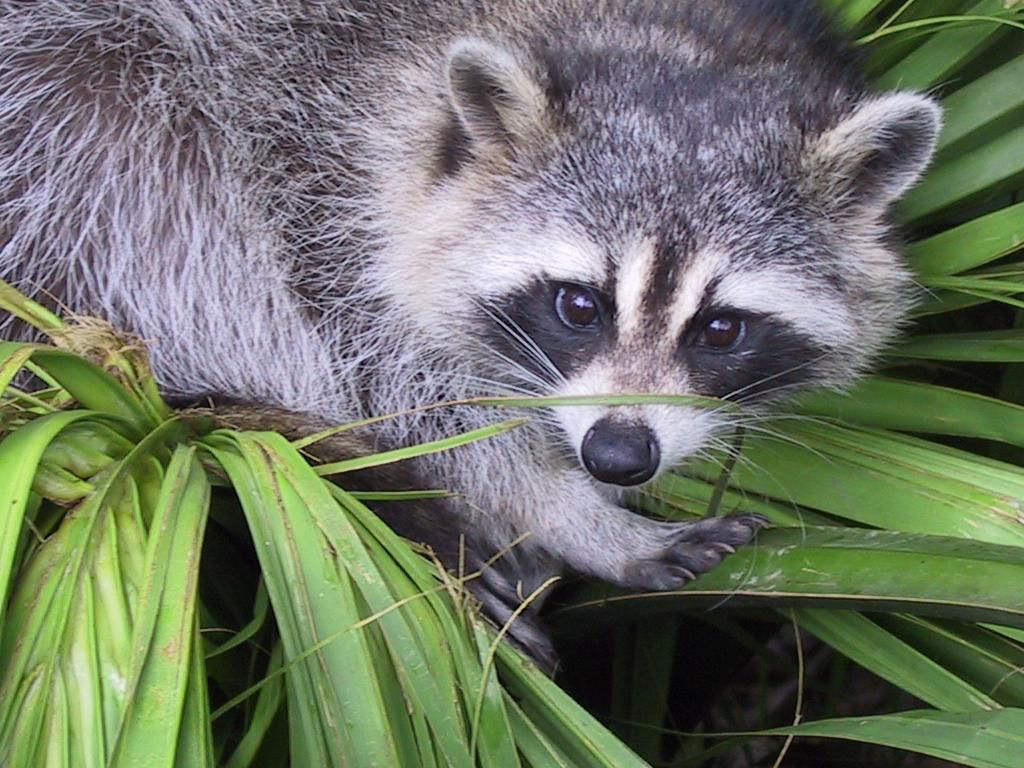
\includegraphics[width=\textwidth]{./pics/color.png}
    \caption{Исходное изображение}
\end{subfigure}
\qquad
\begin{subfigure}{0.46\textwidth}
    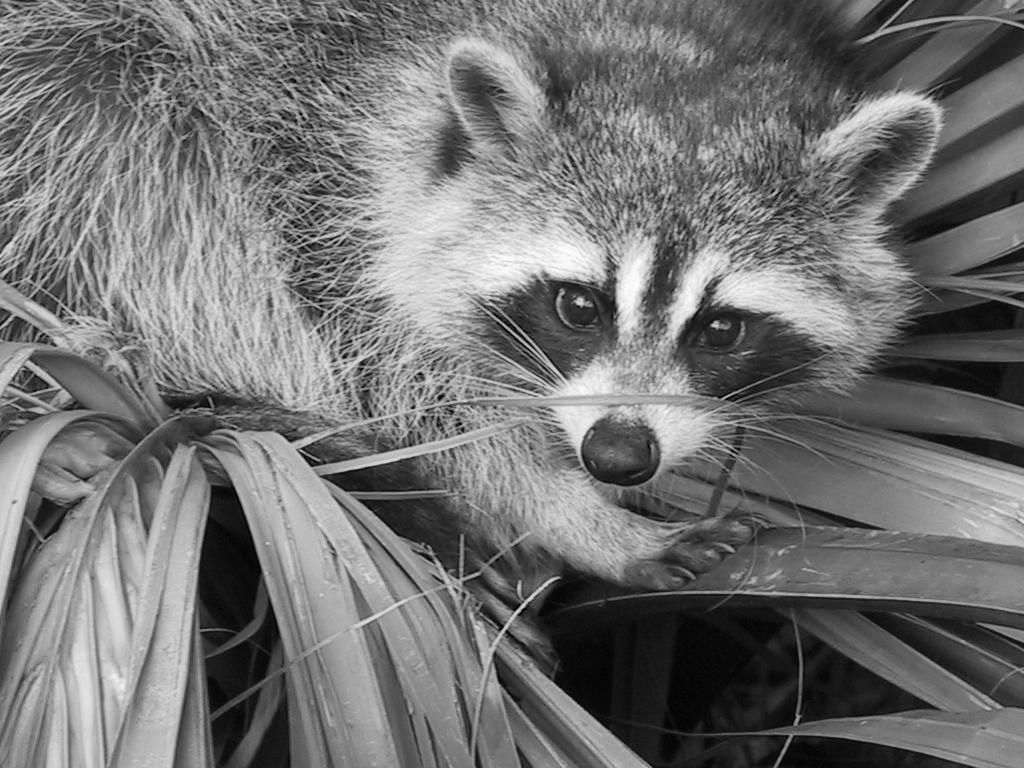
\includegraphics[width=\textwidth]{./pics/gray.png}
    \caption{Результат работы}
\end{subfigure}
\caption{Задача №5. Преобразования цветного изображения в оттенки серого}
\label{pic:task5}
\end{center}
\end{figure}

\analysis

Во всех экспериментах вариант без векторизации выполняется за время, на 2 порядка превосходящее,
время выполнения двух других вариантов. 

Альтернативный вариант имеет преимущетсво перед векторизованным в тех случаях, в которых
количество каналов в изображении мало. Но при увеличении количетсва каналов векторизованный 
вариант становится предподчительнее.


\subsection{Задача №6}

\taskdesc
Реализовать кодирование длин серий (Run-length encoding). Дан вектор \verb"x". Необходимо вернуть кортеж из
двух векторов одинаковой длины. Первый содержит числа, а второй~--- сколько раз их нужно повторить.
Пример: \verb"x = np.array([2, 2, 2, 3, 3, 3, 5])". Ответ: \verb"(np.array([2, 3, 5]), np.array([3, 3, 1]))".

\soldesc\\
\begin{minipage}{\linewidth}
\lstinputlisting[caption={Векторизированный вариант}, label={lst:task6:vect}, firstline=11, lastline=17,]{../task6/task6.py}
\end{minipage}
\begin{minipage}{\linewidth}
\lstinputlisting[caption={Вариант без векторизации}, label={lst:task6:nonvect}, firstline=20, lastline=36,]{../task6/task6.py}
\end{minipage}
\begin{minipage}{\linewidth}
\lstinputlisting[caption={Альтернативный вариант}, label={lst:task6:alt}, firstline=39, lastline=54,]{../task6/task6.py}
\end{minipage}

Векторизованное решение устроенно следующим образом. Функция \verb"np.diff" используется для
нахождения позиций тех элементов массива, значение которых отличается от значения следующего 
элемента (считается, что последний элемент массива не совпадает со следующим за ним). 
Затем из массива выбираются элементы, находящиеся на найденных позициях, и с
помощью \verb"np.diff" вычисляется необходимое количетсво повторений каждого значения как разность
между индексами элементов, имеющих несовпадающие значения.

Альтернативный вариант представляет собой частично векторизованное решение.
\testing
Для сравнения скорсти работы методов генерировался случайный массив размера~\text{n}, содержащий 
целые числа.
Время работы всех вариантов решения для входных данных различного объема представлено в таблице \ref{tbl:task6}.

\begin{table}[!h]
\begin{center}
\large
\begin{tabular}{|c|c|c|c|c|}
\cline{3-5}
\multicolumn{2}{c}{} & \multicolumn{3}{|c|}{Время работы (мс)} \\
\hline
\# & описание~данных & 
\begin{tabular}{c} векторизованный\\вариант \end{tabular} & 
\begin{tabular}{c} вариант \\ без~векторизации \end{tabular} & 
\begin{tabular}{c} альтернативный \\ вариант \end{tabular} \\
\hline
1 & \text{n=10000} & 0.201 & 11.978 & 6.131\\
\hline
2 & \text{n=100000} & 1.588 & 146.886 & 86.245\\
\hline
3 & \text{n=1000000} & 17.307 & 1463.759 & 898.774\\
\hline
\end{tabular}
\caption{Задача №6. Сравнение времени работы}
\label{tbl:task6}
\end{center}
\end{table}

\analysis

Векторизованное решение оказывается заметно эффективнее других вариантов.

Так как в альтернативном варианте второй вызов функции~\verb"np.diff" из векторизованного варианта заменён
на цикл, можно сделать вывод о том, что использование функции~\verb"np.diff" делает решение существено 
эффективнее.

\subsection{Задача №7}

\taskdesc
Даны две выборки объектов~--- \verb"X" и \verb"Y". Вычислить матрицу евклидовых расстояний между объектами.
Сравнить с функцией \verb"scipy.spatial.distance.cdist".

\soldesc\\
\begin{minipage}{\linewidth}
\lstinputlisting[caption={Векторизованный вариант}, label={lst:task7:vect}, firstline=20, lastline=26,]{../task7/task7.py}
\end{minipage}
\begin{minipage}{\linewidth}
\lstinputlisting[caption={Стандартный вариант scipy}, label={lst:task7:scipy}, firstline=12, lastline=17,]{../task7/task7.py}
\end{minipage}
\begin{minipage}{\linewidth}
\lstinputlisting[caption={Альтернативный вариант}, label={lst:task7:alt}, firstline=29, lastline=37,]{../task7/task7.py}
\end{minipage}

В векторизованном варианте вычисления начинаются с нахождения с помощью broadcasting трехмерного тензора 
$Z[i, j, k] = (X[i, k] - Y[j, k])^2$. Затем происходит суммирование полученных значений по $k$ и
вычисление квадратного корня.

В альтернативном варианте для каждой строки матрицы \verb"X" с помощью broadcasting вычисляется
её разность со всеми строками матрицы \verb"Y", затем разности возводятся во вторую степень и суммируются.
Для получения ответа остаётся только извлечь квадратный корень из полученных значнений.

\testing


Для сравнения скорсти работы методов генерировилсь случайные матрицы \verb"X" и \verb"Y" 
c размерами~\text{(n, d)} и \text{(m, d)} соответственно.
Время работы всех вариантов решения для входных данных различного объема представлено в таблице \ref{tbl:task7}.

\begin{table}[!h]
\begin{center}
\normalsize
\begin{tabular}{|c|c|c|c|c|}
\cline{3-5}
\multicolumn{2}{c}{} & \multicolumn{3}{|c|}{Время работы (мс)} \\
\hline
\# & описание~данных & 
\begin{tabular}{c} векторизованный\\вариант \end{tabular} & 
\begin{tabular}{c} стандартный вариант\\ scipy \end{tabular} & 
\begin{tabular}{c} альтернативный \\ вариант \end{tabular} \\
\hline
1 & \text{n=20, m=30, d=10} & 0.097 & 0.061 & 0.564\\
\hline
2 & \text{n=400, m=400, d=2} & 11.009 & 2.593 & 18.966\\
\hline
3 & \text{n=100, m=100, d=10} & 1.103 & 0.300 & 3.510\\
\hline
4 & \text{n=100, m=100, d=100} & 8.048 & 2.216 & 8.166\\
\hline
5 & \text{n=100, m=100, d=500} & 79.720 & 10.846 & 26.725\\
\hline
6 & \text{n=100, m=100, d=1000} & 174.507 & 21.609 & 53.439\\
\hline
7 & \text{n=400, m=400, d=20} & 31.504 & 7.642 & 33.158\\
\hline
8 & \text{n=400, m=400, d=100} & 302.907 & 34.916 & 93.727\\
\hline
9 & \text{n=400, m=400, d=400} & 720.613 & 138.863 & 408.538\\
\hline
10 & \text{n=400, m=400, d=800} & 1372.627 & 284.279 & 974.328\\
\hline
\end{tabular}
\caption{Задача №7. Сравнение времени работы}
\label{tbl:task7}
\end{center}
\end{table}

\analysis

Стандартный вариант scipy демонстрирует наилучшую эффективность. 
Векторизованный вариант оказывается лучше альтернативного при малых значениях \verb"d",
но при больших значениях устапает в скорости. Скорее всего это связано с тем, что
альтернативный вариант при больших \verb"d" использует меньшие объемы памяти.

\subsection{Задача №8}

\taskdesc
Реализовать функцию вычисления логарифма плотности многомерного нормального распределения
Входные параметры: точки \verb"X", размер \verb"(N, D)", мат. ожидание \verb"m", вектор длины \verb"D", 
матрица ковариаций \verb"C", размер \verb"(D, D)". 

Сравнить с \verb"scipy.stats.multivariate_normal(m, C).logpdf(X)" как по скорости работы, так и по точности вычислений.

\soldesc\\
\begin{minipage}{\linewidth}
\lstinputlisting[caption={Векторизованный вариант}, label={lst:task8:vect}, firstline=22, lastline=35,]{../task8/task8.py}
\end{minipage}
\begin{minipage}{\linewidth}
\lstinputlisting[caption={Стандартный вариант scipy}, label={lst:task8:scipy}, firstline=12, lastline=19,]{../task8/task8.py}
\end{minipage}
\begin{minipage}{\linewidth}
\lstinputlisting[caption={Альтернативный вариант}, label={lst:task8:alt}, firstline=38, lastline=53,]{../task8/task8.py}
\end{minipage}

Векторизованное и альтернативное решения вычисляют требуемые значения, используя формулу:
$$
\log{p(x)} = - \frac{d \log{(2\pi)} + \log{|C|} + (x - m)C^{-1}(x-m)^T}{2},
$$
где $x$ ~--- вектор-строка длины $d$, содержащий координаты точки, в которой требуется вычислить логарифм плотности;
$m$ ~--- вектор-строка длины $d$, содержащий математические ожидания и $C$ матрица ковариаций $d \times d$.

Но в векторизоввнном решении последнее слагаемое в числителе дроби вычисляется, при подставлении
вместо x выражения $(x - m)$ и $(x - m)^T$ всех возмножных пар строк матрицы $X$, после чего из полученных
значений выбираются те, которые вычислены для пар, в которых участвовала одна и та же строка.

\testing

Для сравнения скорсти работы методов генерировилсь случайная матрица \verb"X" размера~\verb"(n, d);"
случайные вектор \verb"m" размера~\verb"d" и случайная симметричная положительно определенная 
матрица \verb"C" размера~\verb"(d, d)".
Время работы всех вариантов решения для входных данных различного объема представлено в таблице \ref{tbl:task8}.

\begin{table}[!h]
\begin{center}
\normalsize
\begin{tabular}{|c|c|c|c|c|}
\cline{3-5}
\multicolumn{2}{c}{} & \multicolumn{3}{|c|}{Время работы (мс)} \\
\hline
\# & описание~данных & 
\begin{tabular}{c} векторизованный\\вариант \end{tabular} & 
\begin{tabular}{c} стандартный вариант\\ scipy \end{tabular} & 
\begin{tabular}{c} альтернативный \\ вариант \end{tabular} \\
\hline
1 & \text{n=100, d=10} & 0.484 & 0.589 & 1.105\\
\hline
2 & \text{n=100, d=80} & 6.080 & 5.845 & 4.986\\
\hline
3 & \text{n=100, d=100} & 9.354 & 9.189 & 7.876\\
\hline
4 & \text{n=100, d=400} & 306.027 & 264.812 & 297.941\\
\hline
5 & \text{n=200, d=10} & 1.443 & 0.594 & 1.937\\
\hline
6 & \text{n=200, d=100} & 18.971 & 11.569 & 11.097\\
\hline
7 & \text{n=200, d=200} & 71.188 & 53.179 & 54.177\\
\hline
8 & \text{n=200, d=800} & 2684.795 & 1951.876 & 2553.240\\
\hline
9 & \text{n=2000, d=2} & 56.682 & 0.573 & 17.207\\
\hline
10 & \text{n=2000, d=20} & 197.693 & 2.964 & 19.602\\
\hline
11 & \text{n=2000, d=100} & 980.057 & 54.215 & 71.467\\
\hline
12 & \text{n=2000, d=200} & 2148.684 & 216.427 & 248.340\\
\hline
\end{tabular}
\caption{Задача №8. Сравнение времени работы}
\label{tbl:task8}
\end{center}
\end{table}

Тестовые запуски показали, что резльтаты работы методов совпадают с абсолютной точностью $10^{-5}$.

\analysis

Стандартный вариант scipy демонтсрирует наилучшее время работы. 
Векторизованный вариант работает быстрее альтернативного лишь при достаточно малых
значениях \verb"n" и \verb"d", так как в этом варианте происходят
<<лишние>>   вычисления.

\section{Анализ проделанной работы}

Все задания, описанные в секции \ref{sec:desc} выполнены. 

\begin{itemize}
    \item 
    Для каждой задачи в отдельном модуле написаны три решения, кроме того в модуле для каждой
    задачи реализована функция, генерерующая входные данные для тестовых запусков.
    \item 
    Также для каждой задачи подготовлен модуль, содержащий автоматические тесты для 
    проверки совпадения результатов решений.
    \item 
    В IPython notebook реализована функция для автоматического запуска экспериментов по
    задаче, которая использовалась для сравнения времени работы решений на различных входных
    данных.
    \item
    Коды всех решений, тестов и вспомогательных функций соответствуют style guide PEP 8.
    \item
    Проведен анализ полученных данных и получены выводы.
    \item
    О проделанной работе подготовлен данный отчёт.
\end{itemize}

\section{Заключительные выводы}

Данная работа, показывает что использование библиотеки \verb"numpy" позволяет
значительно повысить эффективность работы программы. Однако, имееют место случаи, в которых
заранее не очевидно какой именно способ решения позволит добиться максимальной производительности.
Полученные результаты свидетельствуют о том, что в таких случаях стоит выбирать способ решения исходя из
ограничений на входные данные в конкретной задаче.


\end{document}
